\documentclass[10pt,a4paper]{article}
\usepackage[utf8]{inputenc}
\usepackage[ruled]{algorithm2e}
\usepackage{fullpage}
\usepackage{graphicx}
\usepackage{float}
% \floatstyle{boxed}
% \restylefloat{figure}
\usepackage[portuguese]{babel}
\usepackage[]{amsmath}
\restylefloat{figure}

\usepackage[adobe-utopia]{mathdesign}
\usepackage[T1]{fontenc}

\usepackage{mdframed}

\DeclareGraphicsExtensions{.jpg,.pdf}

\numberwithin{equation}{section}

\title{TP3: Beating the house!}
\author{Victor Pires Diniz}

\begin{document}
\maketitle
\begin{center}
Algoritmos e Estruturas de Dados III - 1º Semestre de 2015
\end{center}

\begin{figure}[H]
    \centering
    \includegraphics[width=0.90\textwidth]{graphics/cover.pdf}
    \label{fig:cover}
\end{figure}

\section{Introdução}

Algoritmos de força bruta são capazes de alcançar soluções válidas para grande parte dos problemas na ciência da computação. No entanto, esse tipo de solução se torna rapidamente custosa, conforme cresce o tamanho da entrada. Por essa razão, é geralmente interessante procurar por propriedades do problema que permitam a utilização de algoritmos mais específicos e eficientes, através da redução do espaço de busca de solução.

O cenário do trabalho envolve um jogo de cassino no qual o jogador deve tomar uma série de decisões, com pleno conhecimento do cenário do jogo, de forma a otimizar o seu resultado final. De acordo com a história da especificação, o cassino assume que só é possível obter a solução ótima do problema através de força bruta e que, por isso, os jogadores não seriam capazes de vencer com frequência. No entanto, isso não é verdade: o problema de otimização do jogo apresenta propriedades que permitem a aplicação de um algoritmo muito mais eficiente.

São propostos três algoritmos, com desempenhos crescentes. Inicialmente, é utilizado um algoritmo de força bruta, com desempenho ruim para entradas grandes. Posteriormente, é proposta uma solução utilizando programação dinâmica, aproveitando as propriedades do problema. Essa solução apresenta desempenho muito melhor do que a inicialmente obtida, sendo capaz de obter resposta rapidamente para todas as configurações de entrada. Por fim, é paralelizado o algoritmo de programação dinâmica, obtendo-se performance ainda melhor.

\section{Resolução do problema}

O problema do trabalho envolve a otimização das jogadas de um jogo de azar, no qual o jogador recebe uma sequência $S$ de $n$ números inteiros, um valor inicial $I$, um limite $L$ e um patamar de vitória $V$. Esse jogador tem acesso a todos esses valores e deve decidir entre jogar ou não jogar nessa rodada. Caso ele escolha jogar, ele deve seguir a sequência na ordem apresentada, e, para cada número, escolher somá-lo ou subtraí-lo ao valor atual. Se esse valor ultrapassar, a qualquer momento, o limite, ou descer abaixo de zero, o jogador perde imediatamente. Ao final da sequência, se o valor obtido for maior ou igual ao patamar de vitória, o jogador vence. É preciso, portanto, obter a combinação de adições e subtrações que maximiza o valor final a ser obtido. É possível que não haja combinações que permitam a vitória, devido à configuração da entrada.

A saída do problema pede não só se é possível ou não vencer, mas também o maior valor que pode ser obtido, independentemente do resultado do jogo. No caso, apenas valores obtidos ao final da sequência se aplicam. Se não é possível chegar ao final da sequência em uma certa configuração, o programa deve imprimir $-1$ como o valor obtido.

\subsection{Força bruta (\emph{solver\_bf.c})}

O algoritmo de força bruta para esse problema é bastante simples quando feito recursivamente. Partindo do valor inicial, o algoritmo tenta somar e subtrair o próximo valor da sequência ao montante. Caso o valor obtido nessas operações seja válido dentro do intervalo $[0,L]$, são realizadas novas chamadas recursivas com os novos valores como montantes que tentarão adicionar ou subtrair o próximo item da sequência. Se alguma combinação de adições e subtrações for capaz de alcançar o final da sequência, o valor final é comparado com o melhor resultado obtido até então. É utilizada uma variável global auxiliar para armazenar o maior valor final obtido até o momento.

\begin{function}[H]
    % \DontPrintSemicolon
    \caption{recursiveCall($S$, $i$, $n$, $s$, $L$, \&$B$)}

    \KwData{Sequência $S$, posição na sequência $i$, tamanho da sequência $n$, soma parcial $s$, limite superior $L$, melhor valor obtido (global) $B$}
    \KwResult{Ao final, $B$ possuirá o maior valor que pode ser obtido com a sequência fornecida. Caso não haja valores finais válidos, $B$ não é definido nesse procedimento, mantendo seu valor inicial, que é $-1$.}
    \BlankLine

    \If{$s + S[i] \le L$}{
    	\eIf{$i + 1 = n$}{
    		\If{$s + S[i] > B$}{
    			$B \gets s + S[i]$\;
    		}
    	}{
    		\emph{recursiveCall}($S$, $i + 1$, $n$, $s + S[i]$, $L$, \&$B$);
    	}
    }

    \If{$s - S[i] \ge 0$}{
    	\eIf{$i + 1 = n$}{
    		\If{$s - S[i] > B$}{
    			$B \gets s - S[i]$\;
    		}
    	}{
    		\emph{recursiveCall}($S$, $i + 1$, $n$, $s - S[i]$, $L$, \&$B$)\;
    	}
    }
\end{function}

A função acima é chamada inicialmente para o primeiro item da sequência, com a soma inicial sendo o valor inicial $I$.

\subsection{Algoritmo guloso ou programação dinâmica?}

A especificação do trabalho afirma que existe uma maneira eficiente de resolver esse problema utilizando apenas um desses paradigmas. A programação dinâmica e o algoritmo guloso possuem um ponto em comum: ambos dependem da existência de uma subestrutura ótima no problema apresentado. No entanto, eles diferem em como agir em cada fase do problema. Enquanto um algoritmo guloso nunca volta atrás e tenta agir com base em uma decisão local, um algoritmo de programação dinâmica guarda as computações válidas anteriores, caso a melhor opção até então não seja a mais viável para os estados seguintes da entrada.

Com base nisso, é relativamente simples provar que o algoritmo guloso não é ideal para este problema. A melhor combinação até um certo ponto pode não ser a combinação que vai gerar o resultado ótimo para o próximo item da sequência, devido à existência do limite superior. A entrada $S = \{1,2\}, L = 2, I = 1$ é um bom contra-exemplo para a escolha gulosa. Simplesmente somar o maior valor e subtrair quando não for possível somar gera como resultado $0$, mas a solução ótima no caso é subtrair primeiro e somar depois, resultando em $2$. Como se não bastasse, existem situações nas quais o algoritmo guloso falha completamente em obter uma solução. Por exemplo, $S = \{2, 19\}, L = 30, I = 13$: somar o $2$ faz com que não seja possível jogar no segundo turno, levando à derrota imediata.

\subsection{Programaçao dinâmica (\emph{solver\_dp.c})}

Como mencionado, a chave para uma solução de programação dinâmica para esse problema envolve guardar os valores que podem ser obtidos no estado anterior. O que torna o algoritmo de força bruta problemático é o cálculo repetido dos mesmos subproblemas. O armazenamento das somas válidas anteriores permite garantir a unicidade de cada valor e evitar, dessa maneira, a exponencialidade.

\begin{equation}
    V[i]=\begin{cases}
        \{I\}, & \text{se $i = -1$;}\\
        A \cup B \vert \begin{array}{ll}
        	A = a + S[i] \vert \forall a \in V[i-1], a + S[i] \le L \\
        	B = b - S[i] \vert \forall b \in V[i-1], b - S[i] \ge 0
        \end{array}, & \text{caso contrário.}
    \end{cases}
\end{equation}

A equação de recorrência acima representa o conjunto de resultados em cada estado do procedimento. O caso base da recorrência significa que, antes dos itens da sequência serem levados em consideração, o único valor válido é o valor inicial. A recorrência em si tenta somar ou subtrair o item da sequência aos valores válidos do estado anterior. O maior resultado possível no jogo após o estágio $i$ da sequência é o valor máximo presente em $V[i]$.

\begin{algorithm}[H]
    % \DontPrintSemicolon
    \caption{Algoritmo de programação dinâmica}

    \SetKwInOut{Input}{Entrada}
    \SetKwInOut{Output}{Saída}

    \Input{Sequência $S$, tamanho da sequência $n$, valor inicial $I$, limite superior $L$}
    \Output{Melhor resultado possível com a configuração apresentada na entrada, $-1$ caso não haja resultados válidos.}
    \BlankLine
    $A \gets \{I\}$\;
    \ForEach{$p \in S$}{
        $N \gets \emptyset$\;
    	\ForEach{$k \in A$}{
			\If{$k + p \le L$}{
				Insere $k + p$ em $N$\;
			}
			\If{$k - p \ge 0$}{
				Insere $k - p$ em $N$\;
			}
    	}
    	$A \gets N$\;
    }
    \eIf{$A \neq \emptyset$}{
        \textbf{return} \emph{max($A$)}\;
    }{
        \textbf{return} $-1$\;
    }
\end{algorithm}

A implementação dos conjuntos do algoritmo acima foi feita através de dois vetores de valores booleanos de tamanho $L + 1$ (de $0$ a $L$): um para o estado anterior e outro para o novo estado (serão chamados de $A$ e $N$, respectivamente). Se $A[k]$ é \emph{true}, isso significa que $k$ é um valor que pode ser obtido com a adição ou subtração dos valores da sequência até o estado anterior sem sair do intervalo $[0,L]$ em momento algum. Portanto, o algoritmo se torna bastante simples: para cada item da sequência, itera-se por $A$.

\begin{figure}[H]
    \centering
    \includegraphics[width=0.90\textwidth]{graphics/dp.pdf}
    \caption{Demonstração dos estágios do algoritmo de programação dinâmica.}
    \label{fig:dp}
\end{figure}

Para cada $A[k]$ com valor \emph{true}, o próximo item da sequência, $p$, é somado e subtraído a $k$. $N$ inicia a iteração como \emph{false} para todos os índices. $N[k+p]$ e $N[k-p]$ serão \emph{true} desde que $k+p$ e $k-p$ pertençam ao intervalo $[0,L]$, respectivamente. Ao final da sequência, o maior valor que pode ser obtido é o maior valor de $k$ tal que $A[k]=\text{\emph{true}}$, $0 \le k \le L$ ou $-1$, caso $A[k]$ seja \emph{false} para todo $k$.

\subsection{Paralelização do algoritmo de P.D. (\emph{solver\_dp\_p.c})}

O algoritmo de programação dinâmica proposto na seção anterior apresenta oportunidades de paralelismo. Essas oportunidades se restringem a paralelismo de dados, visto que paralelismo de tarefas é inviável, devido à dependência de dados entre cada estágio do procedimento: para processar os valores obteníveis com a adição ou subtração de um item da sequência, é preciso ter terminado de processar os valores da fase anterior.

\begin{figure}[H]
    \centering
    \includegraphics[width=0.90\textwidth]{graphics/parallel.pdf}
    \caption{Demonstração dos estágios do algoritmo de programação dinâmica com paralelismo (exemplo para 4 threads).}
    \label{fig:parallel}
\end{figure}

O paralelismo de dados, nesse caso, é bastante simples, devido à forma como o algoritmo anterior foi implementado. Em particular, a representação do conjunto dos valores da etapa anterior como um vetor de valores booleanos permite paralelizar o processamento de cada etapa por blocagem: o vetor é dividido em $t$ (número de \emph{threads}) partes iguais, e cada \emph{thread} se torna responsável pelo processamento de uma parte. Essa paralelização também é realizável na etapa que zera o vetor dos valores do próximo estágio. Não é necessário fazer grandes modificações no funcionamento do algoritmo em si. Esclarecimentos sobre os detalhes de implementação estão disponíveis diretamente no código-fonte.

\section{Análise de Complexidade Assintótica}

Na análise de complexidade assintótica a seguir, três parâmetros serão usados: o número de itens na sequência ($n$), o número de núcleos disponíveis para processamento paralelo na máquina ($c$) e o limite máximo do jogo ($L$).

\subsection{Força bruta (\emph{solver\_bf.c})}

A abordagem de força bruta cria, potencialmente, duas chamadas recursivas para cada chamada de \emph{recursiveCall}, até que as chamadas alcancem o final da sequência. Isso significa que, no pior caso, esse algoritmo tem complexidade de tempo $O(2^n)$. A complexidade de espaço desse procedimento, por outro lado, é linear, visto que o número máximo de chamadas de \emph{recursiveCall} na pilha em um determinado momento é $n$.

\subsection{Programação dinâmica (\emph{solver\_dp.c})}

O algoritmo de programação dinâmica utilizado aloca vetores proporcionais ao limite máximo do jogo, com $L + 1$ elementos e não realiza chamadas recursivas. Dessa maneira, sua complexidade de espaço é $O(L)$. A função itera para cada item da sequência pelo vetor que representa o conjunto de valores do estágio anterior, de tamanho $L$ e, por isso, realiza $n \times L$ iterações, tendo, assim, complexidade assintótica de tempo $O(nL)$.

\subsection{P.D. em paralelo (\emph{solver\_dp\_p.c})}

Esse algoritmo é muito similar ao algoritmo regular de programação dinâmica, mas o processamento de cada etapa é dividido entre os $c$ núcleos disponíveis, desde que o número de \emph{threads} seja definido apropriadamente. Ainda há, porém, um loop de $L$ iterações não-paralelizado ao final da função principal, cujo papel é descobrir o maior valor após a última etapa. Dessa maneira, a complexidade dessa versão do programa é $O(n \times \frac{L}{c} + L)$. Sua complexidade de espaço continua sendo $O(L)$.

\section{Análise experimental}

Nessa seção, são realizados dois testes. O primeiro deles realiza uma comparação de desempenho entre as versões de força bruta e programação dinâmica, evidenciando a diferença entre a complexidade assintótica desses programas conforme cresce o tamanho da sequência. O segundo teste compara a performance paralela do algoritmo de programação dinâmica em função do número de \emph{threads} alocadas para o programa.

\subsection{Ambiente e metodologia}

Todas as instâncias de teste foram executadas dez vezes cada em uma máquina com as seguintes especificações:

\begin{itemize}
    \item OS: Ubuntu 12.04 LTS x64;
    \item CPU: Intel Core i7 2600 @ 3.40GHz;
    \item RAM: 16GB.
\end{itemize}

Os testes foram realizados no dia 2 de julho de 2015. A medição do tempo de execução de cada instância de teste foi realizada através do comando \emph{time}, no terminal.

\subsection{Teste 1: força bruta vs. programação dinâmica}

O primeiro teste realizado pretende demonstrar o crescimento exponencial da versão de força bruta e compará-lo à versão de programação dinâmica, que cresce linearmente com o aumento do número de itens da sequência. Para isso, foi utilizado um caso de teste com uma sequência que nunca sai do intervalo $[0,L]$, garantindo que haja o máximo possível de chamadas recursivas na versão de força bruta. Além disso, para permitir a comparação das duas versões do programa, o limite superior $L$ foi calibrado para equalizar o tempo de execução do primeiro teste. Isso foi possível porque apenas a versão de programação dinâmica depende desse parâmetro. Os resultados estão disponíveis no gráfico abaixo.

\begin{figure}[H]
\begin{mdframed}
    \centering
    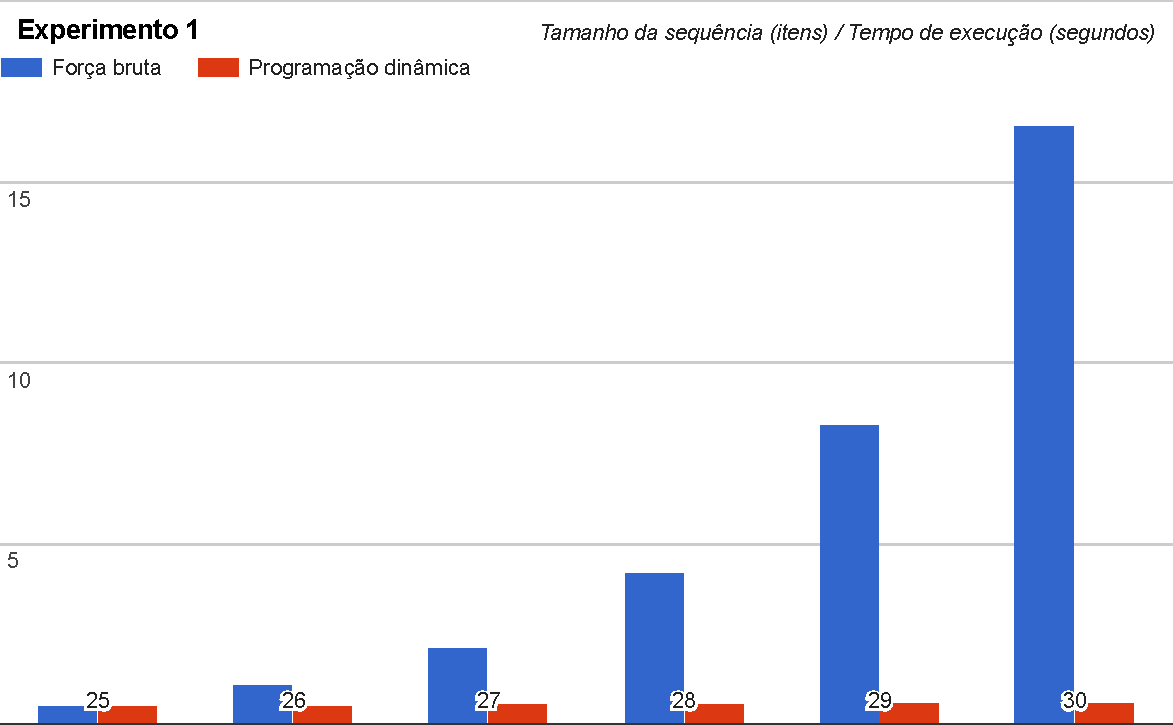
\includegraphics[width=0.90\textwidth]{graphics/exp1_bf.pdf}
    \caption{Gráfico do tempo médio de execução dos testes (em segundos) em função do tamanho da sequência.}
    \label{fig:experimento1}
\end{mdframed}
\end{figure}

O teste se comportou exatamente como previsto. O aumento no número de itens provocou crescimento exponencial do tempo de execução da versão de força bruta do programa, mas apenas crescimento linear na versão de programação dinâmica.

\subsection{Teste 2: sequencial vs. paralelo}

Este segundo teste demonstra o desempenho do programa em função do crescimento do número de \emph{threads} alocadas para a sua execução. É esperado que inicialmente haja melhora na performance com o aumento do número de \emph{threads}, mas que o tempo de execução eventualmente se estabilize e possivelmente comece a crescer. Isso ocorre devido aos ganhos marginais decrescentes de performance conforme cresce o número de \emph{threads} em relação à degradação causada pelos custos de comunicação e outras formas de \emph{overhead} associadas à criação excessiva de \emph{threads}. O gráfico a seguir contém os resultados do experimento.

\begin{figure}[H]
\begin{mdframed}
    \centering
    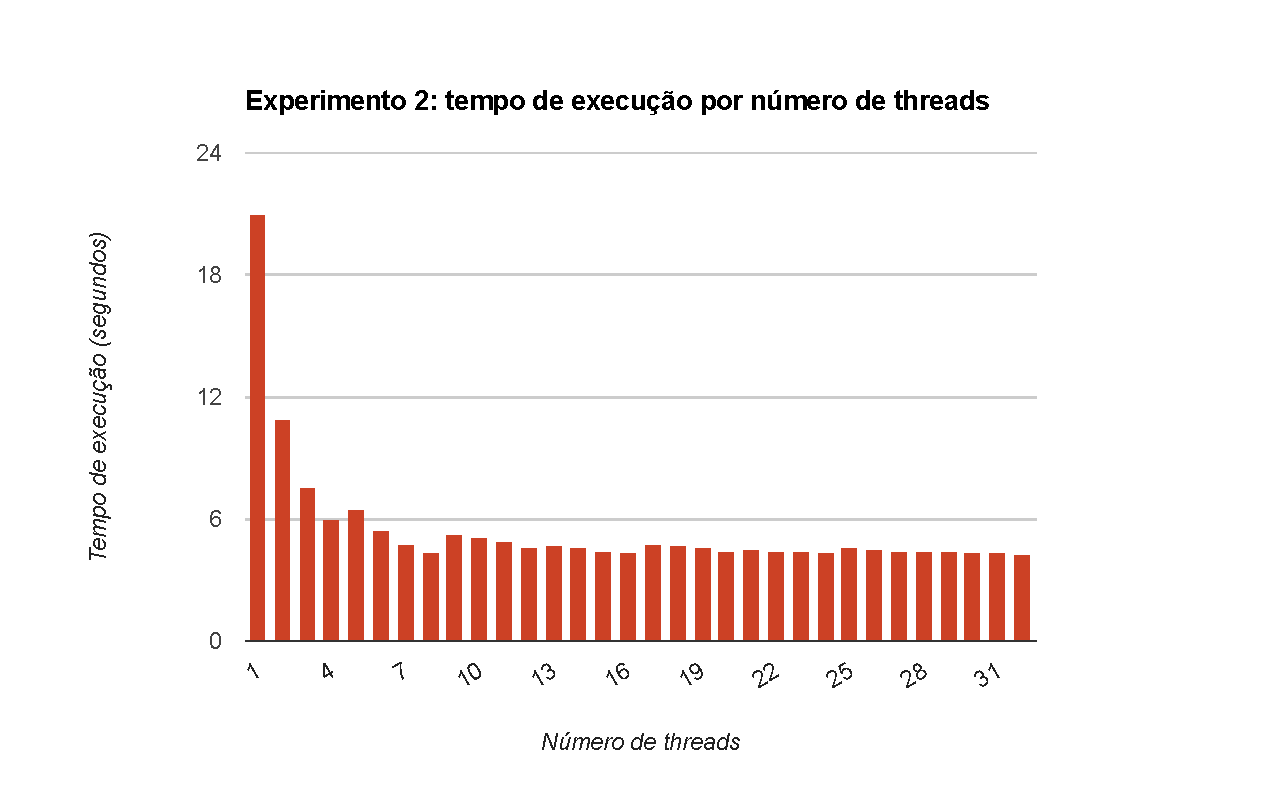
\includegraphics[width=0.90\textwidth]{graphics/exp2.pdf}
    \caption{Gráfico do tempo médio de execução dos testes (em segundos) em função do número de threads utilizadas.}
    \label{fig:experimento2}
\end{mdframed}
\end{figure}

Como previsto, o tempo de execução do teste se estabilizou rapidamente na casa dos 4 segundos, havendo, assim, um speedup aproximado de (levando em consideração o tempo de execução médio dos casos de 1 e 32 threads):

\[
    S = \frac{T_1}{T_32} = \frac{21,16}{4,30} = 4,92
\]

Vale lembrar, porém, que o número ótimo de threads a ser utilizado depende da configuração do teste sendo realizado, do ambiente de execução, entre outros fatores. Nessa implementação, o paralelismo é utilizado para caminhar no vetor utilizado para representar os conjuntos de valores de cada estado do jogo. Portanto, se esses vetores fossem ainda maiores, é possível que aumentar ainda mais o número de threads utilizadas pudesse ser benéfico.

Além disso, com esses dados, é possível analisar o speedup do programa 


\section{Conclusão}

Nesse trabalho, foi solucionado um mesmo problema de diversas formas, de forma a relevar as diferenças entre algoritmos de força bruta e métodos mais especializados para o problema em questão. Além disso, utilizou-se paralelismo para obter ganhos de performance de quase $400\%$. O desempenho de cada versão do programa teve sua performance analisada assintoticamente e a análise realizada foi comprovada através de baterias de testes.

Há várias maneiras de melhorar ainda mais esse programa. A mais notável seria implementar uma representação para os conjuntos na solução de programação dinâmica que independesse do limite superior do jogo. Isso pode ser conveniente em situações nas quais o limite superior possa tomar valores muito grandes ou indefinidos, ou em casos em que os valores da sequência sejam números reais, o que inviabilizaria a representação utilizada. Dentro dos limites propostos para esse trabalho, porém, a implementação realizada é boa o bastante.

\end{document}